\chapter{Considerações finais}
\label{consideracoes-finais}


\section{Resultados}
\label{results}

\subsection{Plugin Ldap UnB}

O plugin que faz comunicação com o Ldap da UnB encontra-se em fase de homolagação
Com o auxilio de uma ferramenta de análise de código para Ruby chamada Rcov, foi obtida a taxa de cobertura de código do plugin desenvolvido, além de alguns dados sobre a execução dos testes funcionais e unitários que seguem abaixo:

\begin{itemize}
\item Quantidade de testes executados: 96 testes
\item Quantidade de assertivas executadas: 111 assertivas
\item Quantiadde de falhas obtidas: 0 falhas
\item Tempo de execução dos testes: 7.8 segundos
\end{itemize}
%
Na imagem abaixo existem dois graficos de cobertura de codigo, o primeiro definido como \textit{'total coverage'} representa a contagem realizada com as linhas em branco e os comentários do código, já o \textit{'code coverage'} representa a contagem realizada sem as linhas em branco e os comentários do código.
%
\begin{figure}[!h]
    \centering
    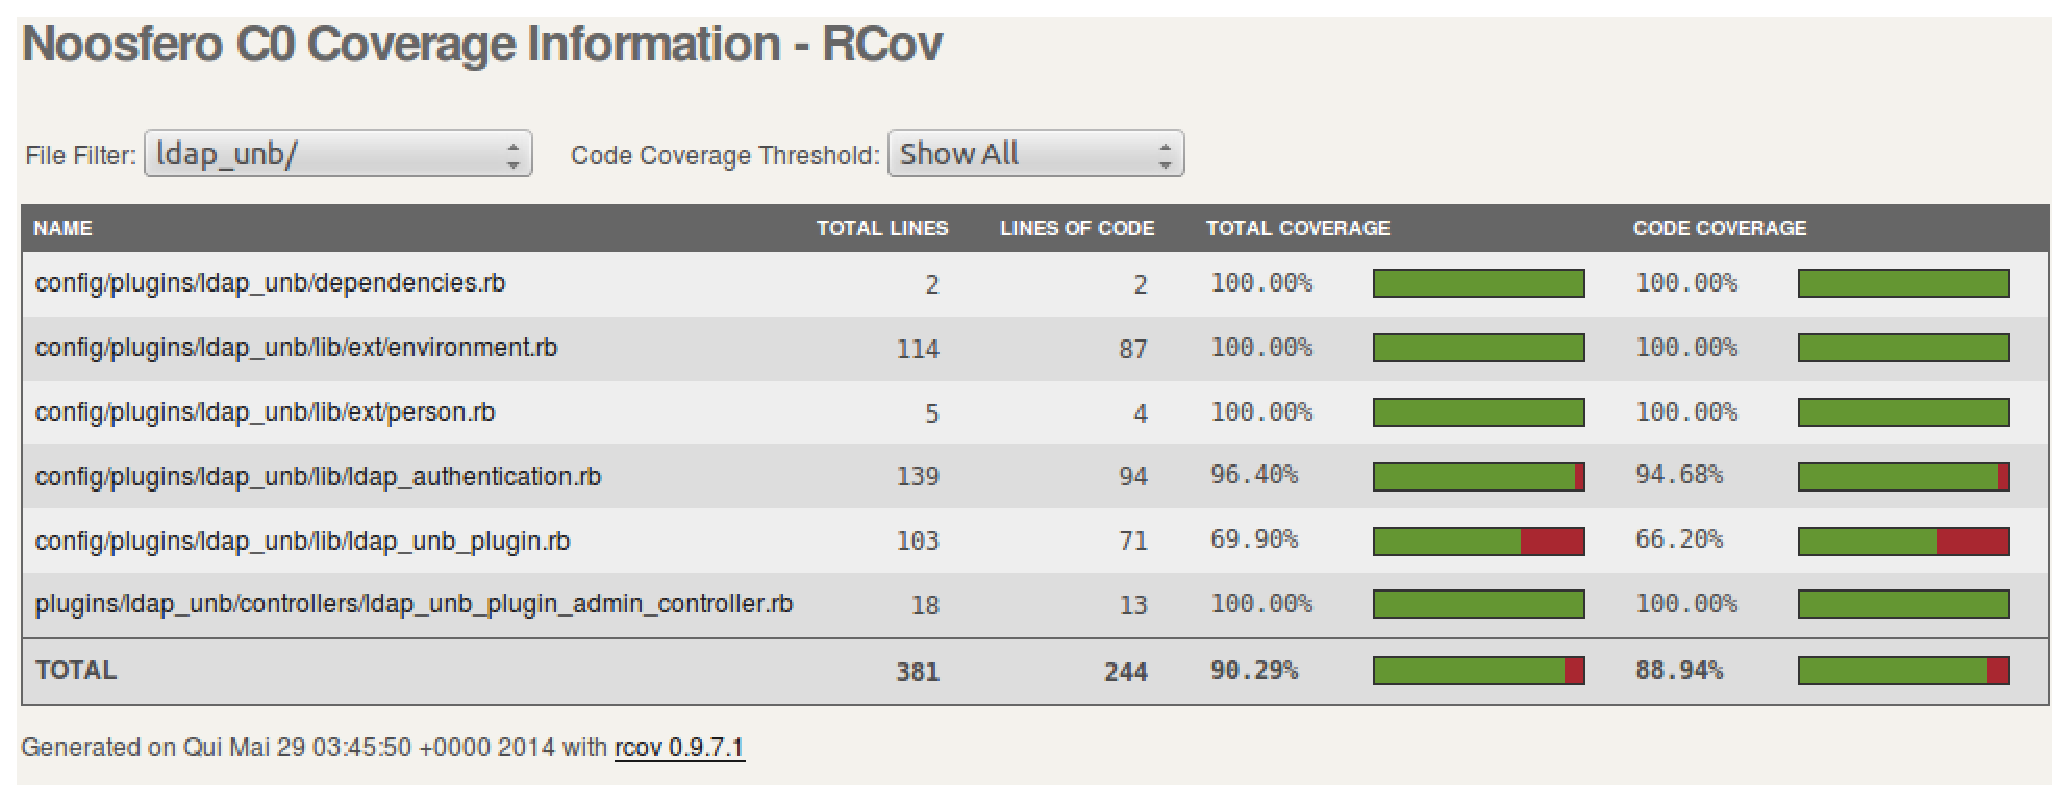
\includegraphics[keepaspectratio=false,scale=0.45]
      {figuras/cobertura_teste.eps}
    \caption{Cobertura de código do Plugin LdapUnb}
    \label{noosfero_bug}
\end{figure}
%

\subsection{Plugin para envio de TCC}

A ferramenta Rcov também foi utilizada para dimensionar a taxa de cobertura de código deste plugin, segue os dados sobre a execução dos testes funcionais e unitários:

\begin{itemize}
\item Quantidade de testes executados: 
\item Quantidade de assertivas executadas: 
\item Quantiadde de falhas obtidas: 
\item Tempo de execução dos testes: 
\end{itemize}

-IMAGEM-

Para este plugin também foram desenvolvidos testes automáticos de aceitação, afim de validar a experiência do usuário em diferentes cenários possiveis:
\begin{itemize}
\item Quantidade de cenários executados: 
\item Quantidade de passos executadas: 
\item Quantiadde de falhas obtidas: 
\item Tempo de execução dos testes: 
\end{itemize}

-IMAGEM-

\section{Propostas Futuras}

